\documentclass{article}
\usepackage[pdftex]{graphicx}
\usepackage{amsfonts}
\usepackage{amsmath}
\usepackage{fullpage}
\usepackage{subcaption}
\usepackage{hyperref}
\usepackage{xspace}

\DeclareMathOperator*{\argmax}{arg\,max}
\DeclareMathOperator*{\argmin}{arg\,min}

%compact numbered lists
\newenvironment{myenumerate}{
	\begin{enumerate}
	\setlength{\itemsep}{1pt}
	\setlength{\parskip}{0pt}
	\setlength{\parsep}{0pt}}{\end{enumerate}
	}

%compact numbered lists
\newenvironment{myitemize}{
	\begin{itemize}
	\setlength{\itemsep}{1pt}
	\setlength{\parskip}{0pt}
	\setlength{\parsep}{0pt}}{\end{itemize}
	}

\newcommand{\athfivek}{\texttt{ath5k}}
\newcommand{\backlogger}{\texttt{Backlogger}}
\newcommand{\batctl}{\texttt{batctl}}
\newcommand{\batmanadv}{\texttt{batman-adv}}
\newcommand{\batmand}{\texttt{batmand}}
\newcommand{\bprd}{\texttt{bprd}\xspace}
\newcommand{\ditg}{\texttt{D-ITG}}
\newcommand{\hellointerval}{\texttt{hello\_interval}}
\newcommand{\helloreader}{\texttt{HelloReader}}
\newcommand{\hellowriter}{\texttt{HelloWriter}}
\newcommand{\iproute}{\texttt{iproute2}}
\newcommand{\iptables}{\texttt{iptables}}
\newcommand{\iwconfig}{\texttt{iwconfig}}
\newcommand{\iwlist}{\texttt{iwlist}}
\newcommand{\iwscan}{\texttt{iwscan}}
\newcommand{\iw}{\texttt{iw}}
\newcommand{\libnetfilterqueue}{\texttt{libnetfilter\_queue}}
\newcommand{\libnlroute}{\texttt{libnl-route}}
\newcommand{\libnl}{\texttt{libnl}}
\newcommand{\libpacketbb}{\texttt{libpacketbb}}
\newcommand{\madwifi}{\texttt{madwifi}}
\newcommand{\main}{\texttt{Main}}
\newcommand{\nfqueue}{\texttt{NFQUEUE}}
\newcommand{\ntp}{\texttt{NTP}}
\newcommand{\olsrd}{\texttt{olsrd}}
\newcommand{\releaseinterval}{\texttt{release\_interval}}
\newcommand{\router}{\texttt{Router}}
\newcommand{\updateinterval}{\texttt{update\_interval}}
\newcommand{\wext}{\texttt{wext}}
\newcommand{\wirelesstools}{\texttt{wireless-tools}}

\newcommand{\etal}{\textit{et al.}}

%compact SINR, should be used in a math environment
\newcommand{\sinr}{\textrm{SINR}}
\newcommand{\snr}{\textrm{SNR}}
\newcommand{\rssi}{\textrm{RSSI}}

%compact BER, should be used in a math environment
\newcommand{\ber}{\textrm{BER}}

%circled numbers
\usepackage{tikz}
\newcommand*\circled[1]{\tikz[baseline=(char.base)]{
                \node[shape=circle,draw,inner sep=2pt] (char) {#1};}}

\begin{document}
\thispagestyle{empty}

\title{COTS-BPRD:\\Commercial Off-The-Shelf Backpressure Routing Daemon}
\date{\today}
\author{Jeffrey Wildman and Bradford Boyle\thanks{The authors can be reached at \texttt{jeffrey.wildman@gmail.com} and \texttt{bradford.d.boyle@gmail.com}, respectively.}}

\maketitle


%==============================================================================
\section*{Overview}\label{sec:overview}

COTS-BPRD (\bprd) is a backpressure-inspired routing daemon targeted at commercial-off-the-shelf Linux-based systems with IEEE 802.11 wireless networking capabilities.
Based on a wide body of research literature, backpressure routing strategies are roughly centered around forwarding schemes that dynamically route traffic away from areas of high congestion along congestion gradients.
\bprd consists of a network layer approach to backpressure routing and is implemented as a multi-threaded user-space program written in C.
Key dependencies/features of \bprd include:
\begin{myitemize}
  \item \libnl\ for dynamically querying and configuring network interfaces,
  \item \iptables\ and \libnetfilterqueue\ for capturing/releasing packets and tracking commodity congestion levels,
  \item \libpacketbb\ for reading and writing hello messages that communicate congestion levels between neighboring nodes, and
  \item \libnlroute\ for dynamically querying and configuring each node's routing table.
\end{myitemize}


This document\footnote{The majority of this document was written during the first half of 2012, and as such the review of literature, operating system, drivers, software, etc. may be outdated!} contains a discussion of traditional backpressure routing, related practical implementation issues, and a design overview of \bprd.

\newpage

\setcounter{tocdepth}{2}
\tableofcontents
\newpage


%==============================================================================
\section{Introduction}\label{sec:introduction}

Backpressure routing is roughly characterized by a forwarding policy that direct packet flows (commodities) from network areas of high congestion levels to those with lower congestion in an effort to deliver packets.
Congestion gradients are computed between neighboring routers in the network by tracking commodity backlog levels at each node and measuring the difference in backlog levels across devices (a backlog differential).
The backlog and resulting differentials of one or more commodities (uniquely classified by source, destination, port, etc.) may be tracked independently.
Theoretical backpressure routing provides mechanisms for selecting joint schedules and routes for tracked commodities based on relative backlog differentials and channel conditions present within the network.


This project focused on implementing a decentralized backpressure-inspired routing protocol on a single-board computer (SBC) with wireless networking capabilities.
Single-board computers consist of a single circuit board containing a processor, memory, and various input and output ports in a low-cost, low-power package -- ideal for rapid-prototyping of networking protocols.
To this end, we have produced an experimental implementation of backpressure routing, \bprd.
\bprd incorporates commodity tracking, local backlog information dissemination, and backlog-based routing tables at the network layer, and exists and operates independently on top of the underlying IEEE 802.11 interfaces of the SBC platform.


The rest of this document is organized as follows.
Section~\ref{sec:related-work} discusses related backpressure implementation work in research literature, as well as current mesh and routing protocol development projects.
Section~\ref{sec:hardware} discusses the SBC hardware that has been selected for this implementation effort.
Section~\ref{sec:software} provides an overview of the operating system that has been chosen for development, as well as prominent tools and libraries used to configure and manage network communication.
Section~\ref{sec:theory} provides a recap of the theoretical presentation of backpressure routing, while Section \ref{sec:practice} lists the assumptions of backpressure routing that will need to be addressed in a practical environment and how our implementation addresses these assumptions.
Section~\ref{sec:sample-experiment} discusses a sample experimental setup for a simple network topology.
Section~\ref{sec:future} provides ideas for future work.
Finally, Appendix~\ref{sec:topology} details several techniques that were employed to construct non-full-mesh topologies within a reasonable physical space.



%==============================================================================
\section{Related Work}\label{sec:related-work}

Concerning backpressure-inspired scheduling policies and their implementation, much work has been published in research literature that makes use of legacy (IEEE~802.11) hardware.
Many implementations look to influence the IEEE~802.11 scheduling algorithm either by dynamically changing the protocol's contention window size or by pre-defining a map between priority levels and contention window sizes.
This is often combined with a custom protocol that operates at a higher layer (network and/or transport layer), tracks backlog between nodes, and assigns priority levels to packets as they get passed down the stack.
In the following, we provide an overview of related research literature and further categorize the implementation approaches that we considered.


%==============================================================================
\subsection{Backpressure-Inspired Networking}\label{sec:rel-work-backpressure}

Utility-Optimal CSMA (UO-CSMA), proposed by Lee, \etal\ \cite{LeeLeeYi2009} is a message-free scheduling protocol that theoretically maximizes network utility as a function of network throughput.
Efforts have been made to implement UO-CSMA in legacy wireless systems (IEEE~802.11 wireless systems) using GloMoSim simulator models that run over top of IEEE~802.11 hardware within the programming environment Common Code Architecture (CCA).
Modifications to IEEE 802.11 include dynamic adjustments to contention window sizes and link hold-times, which allow a sender to retain the channel for multiple packets in a row.


A joint scheduling and congestion control algorithm proposed by Akyol, \etal\ \cite{AkyAndGup2008} solves a network utility maximization problem, where utility is a function of the data flow rates in the network.
The proposed algorithm sits above the MAC layer and also relies on contention window adjustments to enforce traffic priorities.
Queue/backlog information is exchanged by including this information with pre-transmission Request-to-Send/Clear-to-Send (RTS/CTS) messages or within data packets and their acknowledgements.
Congestion control mechanisms are built over both UDP and TCP to control the flow of data to lower layers.
This is implemented and simulated in an OPNET model.


DiffQ \cite{WarJanHa2009} is a backlog-based congestion controller implemented between the network and transport layers.
It makes use of the traditionally-unused IP Type-of-Service packet header field to indicate traffic priority which maps to a contention window size at the MAC layer to influence scheduling.
However, DiffQ does not control routes or next-hop decisions; it is assumed a routing protocol (e.g., OLSR) operates underneath DiffQ.
DiffQ is comprised of a module for the Linux 2.6.18 kernel and extended MadWifi drivers that allow up to eight different traffic priority/contention window mappings.
We assume that DiffQ transmits backlog information between neighbors at the transport layer.


Huang, \etal\ \cite{HuaMoeNee2011} investigate using last-in-first-out (LIFO) queueing with backpressure-based scheduling to achieve near-optimal tradeoffs between network utility (throughput) and delay.
This effort is validated with experiments using the Backpressure Collection Protocol (BCP) of \cite{MoeSriKri2010}.
BCP is designed for sensor networks that need to aggregate data to a central collection point and runs on TinyOS, an event-based operating system that supports a variety of sensor mote hardware platforms.


Ryu, \etal\ implement a backpressure-algorithm on a Linux-based IEEE~802.11 testbed by modifying MadWifi drivers to support multiple priority levels (contention windows) and developing a routing algorithm using Click.
The authors focus on modifications to traditional backpressure algorithms to better support intermittently connected networks \cite{RyuBhaPai2010}.


Szwabe, \etal\ \cite{SzwLisNow2010} extend OLSR to support multi-route forwarding and max-weight scheduling.
This was accomplished initially using Click, but was eventually redone within a kernel module.
The max-weight scheduler is used to select next-hop routes for each packet, which are then passed to the underlying IEEE~802.11 layer, which remain unmodified.


Correspondingly, due to the degree of difficulty, few efforts were found that extensively modified IEEE~802.11 drivers.
Laufer, \etal\ \cite{LauSalLun2011} detail a backpressure implementation that involved converting the IEEE~802.11 layer to a TDMA-based access scheme.
During a TDMA frame, a centralized scheduler controls interference estimation to generate a conflict graph, guides passage of queue backlog information, and solves the max-weight-independent-set problem.
The work appears remarkably complete in that great effort was made to satisfy the assumptions of traditional backpressure as much as possible.


%==============================================================================
\subsection{Implementation Approaches}\label{sec:rel-work-impl-approaches}

There were several approaches considered when implementing our backpressure-like routing protocol.
Each of these approaches is highlighted by current, active development projects that make use of them.


The Optimized Link-State Routing Daemon (\olsrd) \cite{olsrd} project is a user-space mesh networking protocol that operates at Layer~3 and implements the Optimized Link State Routing (OLSR) standard \cite{olsr-rfc}.
The Better Approach To Mobile Ad hoc Networking (BATMAN) \cite{batman} project also supplies a user-space daemon (\batmand) mesh networking protocol implementation.
All messaging is done on top of the MAC layer, and as a result, these protocols can run on networks with a wide variety of IEEE~802.11 wireless network cards and Ethernet devices.


Another part of the BATMAN project is \batmanadv, a Layer~2 version implementation of the BATMAN protocol.
This implementation defines its own Ethertype and sends out mesh routing control information encapsulated in Layer~2 frames.
It comes with configuration tools \batctl\ that assist in setting up \batmanadv\ on a variety of interface types (Ethernet, WiFi).
Additionally, the in-progress IEEE~802.11s draft amendment will add mesh networking support directly to the IEEE~802.11 standard.
Under the \texttt{open80211s} project \cite{open80211s}, an open reference implementation of the draft is already available within the Linux kernel and uses a Hybrid Wireless Mesh Protocol (HWMP) that incorporates proactive and reactive routing features.
Both of these projects operate at Layer 2; \batmanadv\ can operate over multiple interface types, while \texttt{open80211s} operates within the confines of the IEEE~802.11 protocol.
A Layer~2 implementation is agnostic to IP addressing and transport protocols, in addition to being closer to available physical layer statistics.


Overall, a Layer~2 implementation would likely require extensive kernel-space development, prolonging initial development and testing.
Additionally, the Layer~2 protocol (IEEE 802.11) supported by our testbed hardware would require several concessions to relax theoretical backpressure assumptions anyway, these are detailed in Section~\ref{sec:practice-issues}.
By choosing a Layer~3 implementation, we not only isolate Layer~2 issues from our backpressure-inspired routing protocol, but also potentially expand the MAC layer protocols on top of which \bprd might be tested and deployed.


%==============================================================================
\section{Hardware}\label{sec:hardware}

\bprd development was performed on a network of PC Engines ALIX.3D3 single-board computers \cite{alix3d3}, each equipped with an Atheros-based wireless networking card \cite{dcma82}.
Each ALIX.3D3 board (shown in Figure~\ref{fig:alix3d3-board}) contains an x86-compatible AMD Geode CPU and is capable of running either Windows or one of several Linux distributions\footnote{The AMD Geode LX 800 requires a non-PAE 32-bit Linux kernel \url{http://www.phoronix.com/scan.php?page=news_item&px=MTAxMzU}}.
Among other features, the ALIX.3D3 board houses \(256\)~MB RAM, one Ethernet port, a CompactFlash socket for operating system and data storage, and two miniPCI slots.
The employed Atheros wireless cards contain an Atheros AR5413 chipset, which supports IEEE~802.11a/b/g standards with speeds up to \(54\)~Mbps (\(108\)~Mbps~Turbo), and are capable of operating on either \(2.4\)~GHz or \(5\)~GHz ISM bands.

\begin{figure}[!ht]
\centering
\null\hfill%
\includegraphics[width=0.45\textwidth]{img/alix3d3.jpg}%
\hfill%
\includegraphics[width=0.45\textwidth]{img/alix3d3b.jpg}%
\hfill\null%
\caption{ALIX.3D3 Board - front side (left) and back side (right) \cite{alix3d3}}
\label{fig:alix3d3-board}
\end{figure}

%==============================================================================
\section{Operating System/Software}\label{sec:software}

Beyond motivating factors such as OS familiarity, the processing and memory specifications of the ALIX.3D3 favor a lightweight Linux distribution over Windows for development and testing of \bprd.
During development, we used Ubuntu 11.10 32-bit Server, but have since updated \bprd to compile on Ubuntu 14.04 64-bit Server.
In the rest of this section, we enumerate drivers, software tools, and libraries used to configure and run \bprd.
This section is meant to be a high-level overview of such software --- the particular usage of software/libraries within \bprd is detailed in Section~\ref{sec:practice-implementation}.


%==============================================================================
\subsection{Drivers}\label{sec:drivers}

To our knowledge, there are currently two open-source Linux-based drivers for our Atheros-based wireless card: \madwifi\ \cite{madwifi} and \athfivek\ \cite{ath5k}.
The last version of \madwifi\ drivers (v9.0.4) was released in February~2008.
Development on \madwifi\ has essentially stopped in favor of the \athfivek\ drivers; during this transition, the \athfivek\ drivers were picked up for inclusion into the Linux kernel (April 2008) \cite{linuxnews} and are under active development.
As a result, the \athfivek\ drivers are preinstalled by Ubuntu and ready to use.
Correspondingly, we made use of the \athfivek\ drivers in our ALIX.3D3 testbed.


%==============================================================================
\subsection{Tools}\label{sec:tools}

There were several software tools used to configure the SBCs.
Each of these is detailed below.

\begin{myitemize}

\item \textbf{\iwconfig}:
  Ignoring graphical-based tools, Wireless Tools \cite{wt} is perhaps the most common tool used
to configure wireless cards.
  Wireless Tools is a collection of command-line programs (\iwconfig, \iwlist, \iwscan, etc.) that allow one to configure a wireless card from userspace.
  The package makes use of the Wireless Extensions API; its last version (v29) was released in September, 2007.
  New hardware can be configured and accessed by these tools via drivers that implement this API.
  The Wireless Tools utilities can be easily installed in Ubuntu by package \wirelesstools.

\item \textbf{\iw}:
  \iw\ is another wireless card configuration tool that has been developed to take advantage of the newer netlink-based wireless card configuration API provided by \texttt{cfg80211} and \texttt{nl80211} \cite{iw}.
  The Linux Wireless developers are actively developing \iw\ and the tool is intended to replace the suite of utilities provided by Wireless Tools (i.e., \iwconfig, et al.).
  While \iw\ allows configuration of mesh-networks on wireless cards supporting it (unlike \iwconfig), transmission power control is still a missing feature from \iw.
  \iw\ can be easily installed in Ubuntu by package \iw, but compiling from the latest version tarball is recommended for Ubuntu 11.10.

\item \textbf{\iptables}:
  \iptables\ \cite{iptables} is a software tool to control Linux packet filtering from userspace.
  \iptables\ is installed in Ubuntu by default.

\item \textbf{\iproute}:
  \iproute\ \cite{iproute2} is a suite of netlink-based Linux networking utilities that covers address configuration, link configuration, routing tables, neighbors (ARP table), etc.
  \iproute\ can easily be installed in Ubuntu by package \iproute.

\item \textbf{\ntp}:
  The Network Time Protocol (\ntp) can be used to synchronize the clocks of computers over a network \cite{ntp}.
  During our experimentation with the ALIX.3D3 boards, it was observed that the onboard clocks were inaccurate and were gaining or losing approximately five minutes over the course of a 24 hour period.
  Left alone, the lack of clock synchronization would have made it difficult to calculate one-way delay and match up trends in experimental data collected at different nodes in the testbed.
  By installing \ntp\ on each SBC and configuring it to synchronize to a pool of servers, we were able to obtain clock offsets less than \(20\) ms between pairs of ALIX.3D3 boards.

\item \textbf{\ditg}:
  The Distributed Internet Traffic Generator (\ditg{}) software package can be used to generate and measure traffic across a network testbed \cite{d-itg}.
  While there are numerous traffic generation tools, \ditg was used because it is able to replicate appropriate stochastic processes for inter-departure time and packet size for traffic generated at the network layer and above.
  Additionally, \ditg provides a tool for measuring the bitrate, packet loss, delay, and jitter for multiple flows.

\end{myitemize}


%==============================================================================
\subsection{Libraries}\label{sec:libraries}

There were several libraries that provided useful functionality or interfaces into the kernel.
Each of these is detailed below.

\begin{myitemize}

\item \textbf{\libnl} \& \textbf{\libnlroute}: The netlink core library \libnl\ provides sockets-like communication
between processes, particularly between the kernel and userspace.
  Additional libraries implement specific portions of the netlink protocol as higher-level interfaces overtop of \libnl.
  In particular, \libnlroute\ provides an interface to set and get the configuration of addresses, interfaces, routes, neighbors, and traffic control \cite{libnl}.

\item \textbf{\libnetfilterqueue}: The \libnetfilterqueue\ library provides an API for accessing, manipulating, and
returning packets caught by \iptables\ filters \cite{libnfq}.

\item \textbf{\libpacketbb}: \libpacketbb\ is a library written by Henning Rogge.
  It can be found within the `olsrv2' git branch of the \olsrd\ open source implementation of the Optimized Link State Routing (OLSR) protocol \cite{olsrd}.
  \libpacketbb\ is a still-in-development implementation of a packet reader/writer that adheres to RFC~5444.
  RFC~5444 specifies a generalized packet format for mobile ad hoc networks \cite{packetbb-rfc}.

\end{myitemize}


%==============================================================================
\section{Theoretical Backpressure Routing}
\label{sec:theory}

Backpressure Routing (originally termed the Maximum Throughput Policy) was established by Tassiulas and Ephremides \cite{TasEph1992} and further explored by many others \cite{GeoNeeTas2006, NeeUrg2009}.
Detailed by Georgiadis, Neely, and Tassiulas \cite{GeoNeeTas2006}, the `max-weight adaptive back-pressure' policy makes routing decisions in a time-slotted network with multi-commodity flows by observing the backlog of each commodity throughout the network.
In a sense, backpressure routing directs packets along per-commodity congestion gradients until they reach their destination (locations of zero-backlog).
In theory, backpressure routing is an optimal control policy, in that it stabilizes the network's backlog for a range of traffic arrival rates (called the \emph{capacity region}) that surpasses that of all other routing control policies.
In this section, we first overview key concepts and equations governing backpressure routing as presented in theoretical research and follow this with a discussion of research efforts to implement backpressure routing and issues expected in practice.


%==============================================================================
\subsection{Terminology}\label{sec:theory-terminology}

Consider a communications network consisting of a set \(\mathcal{N}\) of nodes and \(\mathcal{L}\) of directed links.
A link \((a,b) \in \mathcal{L}\) denotes a communication channel from node \(a \in \mathcal{N}\) to node \(b \in \mathcal{N}\).
Let \(\mathcal{K}\) be a set of commodities, or data flows, defined at the very least by each of the data flows' destination.
In a slotted time system, slot \(t\) refers to the time interval \([t,t+1)\).
The capacity, or transmission rate, of each link \((a,b)\) during slot \(t\), is represented as a function \(C_{ab}(I(t),S(t))\).
Here, \(I(t)\) and \(S(t)\) encompass controllable and uncontrollable factors that affect link capacity.
More formally, \(S(t)\) represents the \emph{topology state process} during slot \(t\).
\(S(t)\) can incorporate factors such as node positions, fading effects, and weather patterns.
\(I(t)\) represents the \emph{control decision variable} that can incorporate factors such as link activation, transmission power, and modulation and coding schemes.
The control decision variable resides in the state space \(\mathcal{I}_{S(t)}\), which may or may not be dependent on the topology state process.
So, at time-slot \(t\), the network controller observes topology state \(S(t)\) and makes a control decision \(I(t)\) that yields link capacities \(C_{ab}\).


%==============================================================================
\subsection{Routing Constraints}\label{sec:theory-routing-constraints}

In addition to determining the link capacities, the network controller must also decide which commodities to route over activated links in the network.
The \emph{routing control variables}, \(\mu_{ab}^{(c)}(t)\), denote the amount of commodity \(c \in \mathcal{K}\) data transmitted over link \((a,b)\) during time-slot \(t\).
The routing control variables are subjected to link capacity constraints such that the sum total of all commodities transmitted over each link during a time-slot does not exceed that link's capacity:
%
\begin{equation}
\label{eq:link-cap-constraint}
\sum_{c\in\mathcal{K}}\mu_{ab}^{(c)}(t) \leq C_{ab}(I(t),S(t))
\end{equation}


Additionally, there may be per-commodity routing constraints that limit which links a commodity may be transmitted over.
Here, \(\mathcal{L}_c \subset \mathcal{L}\) represents the set of links that commodity \(c\) may be sent over:
%
\begin{equation}
\label{eq:link-routing-constraint}
\mu_{ab}^{(c)}(t) = 0 \quad \textrm{if } (a,b) \notin \mathcal{L}_c.
\end{equation}


Finally, note that the routing control variables may be chosen in such a way that not enough of a particular commodity resides at a node to satisfy all outgoing transmissions.
In this case, idle fill bits are transmitted in place of the desired commodity to fulfill the routing control variables.


%==============================================================================
\subsection{Queueing Dynamics}\label{sec:theory-queueing}

Exogenous arrival processes, marked as \(A_{i}^{(c)}(t)\), exist for each commodity \(c\) at each node \(i\).
The variable \(U_i^{(c)}(t)\) marks the commodity \(c \in \mathcal{K}\) backlog at node \(i \in \mathcal{N}\) at time \(t\).
Incorporating the routing control variables discussed above, the backlog queues in the network evolve according to the following relation:
%
\begin{equation}
\label{eq:queue-evolution}
U_{i}^{(c)}(t+1) \leq \max\left[U_{i}^{(c)}(t) - \sum_{b\in\mathcal{N}}\mu_{ib}^{(c)}(t),0\right] + A_{i}^{(c)}(t) + \sum_{a\in\mathcal{N}}\mu_{ai}^{(c)}(t).
\end{equation}


This equation implies the following order of operations: Start with the commodity \(c\) backlog at node \(i\) at time \(t\).
Any outgoing commodity \(c\) transmissions from node \(i\) are first subtracted from node \(i\)'s backlog.
(Note, the maximum is required because there may not be enough commodity \(c\) data to satisfy the routing control variables \(\mu_{ib}^{(c)}(t)\) and the resulting backlog cannot be negative.)
After outgoing transmissions are satisfied, the backlog is augmented by exogenous arrivals and incoming transmissions during slot \(t\).
(Note, the inequality results from the fact that the routing control variables \(\mu_{ai}^{(c)}(t)\) may contain idle fill bits if the respective source nodes did not contain enough commodity \(c\) data to send.)


%==============================================================================
\subsection{Algorithm}\label{sec:theory-algorithm}

During each time-slot, the network controller performs the following actions in an attempt to stabilize the network.

\begin{myenumerate}
\item Observe the topology state \(S(t)\) as well as the backlog at each node for each commodity \(U_{i}^{(c)}(t)\).


\item For each link, denote the \emph{optimal commodity}, \(c_{ab}^{*}(t)\), as the commodity with the largest backlog differential:
%
\begin{equation}
\label{eq:opt-commodity}
c_{ab}^{*}(t) \equiv \arg\max_{c|(a,b)\in \mathcal{L}_c}\left[U_{a}^{(c)}(t) - U_{b}^{(c)}(t)\right],
\end{equation}
%
and let \(W_{ab}^{*}(t)\) be the backlog differential associated with the optimal commodity:
%
\begin{equation}
\label{eq:opt-weight}
W_{ab}^{*}(t) \equiv \max\left[ U_{a}^{(c_{ab}^{*}(t))}(t) - U_{b}^{(c_{ab}^{*}(t))}(t) \right].
\end{equation}


\item Choose the control decision variable \(I(t)\) such that the weighted throughput is maximized:
%
\begin{equation}
\label{eq:bp-opt-problem}
\max_{I(t)} \sum_{(a,b)\in\mathcal{L}} W_{ab}^{*}(t)C_{ab}(I(t),S(t)).
\end{equation}


\item Finally, assign the routing control variables \(\mu_{ab}^{(c_{ab}^{*})}(t) = C_{ab}(I^{*}(t),S(t))\) for links with \(W_{ab}^{*}(t) > 0\).
\end{myenumerate}


%==============================================================================
\section{Practical Backpressure Routing}\label{sec:practice}

In this section, we discuss practical issues that arose when developing our backpressure-inspired routing protocol, and how our implementation addressed such issues.
Additionally, a structural description of our implementation is provided.
We make effort to relate both the practical issues and implementation back to the original theoretical presentation of backpressure routing.


%==============================================================================
\subsection{Issues}
\label{sec:practice-issues}

Backpressure routing as presented in theoretical discussions makes many model assumptions that must be relaxed when considering the algorithm's practical implementation on the targeted SBC hardware.
We make an effort to characterize these assumptions, specify whether they are satisfied by the chosen hardware platform, and what concessions must be made as a result.


\subsubsection{Medium Access Control Layer}

Ideal backpressure assumes the existence of a centralized scheduler that can find the optimal solution to the NP-hard optimization problem in Step~3 above.
Without further simplifying assumptions, the computational burden of solving (\ref{eq:bp-opt-problem}) will quickly overwhelm the capabilities of the SBC hardware for non-trivial networks of sufficient size.
Aside from computational barriers of solving (\ref{eq:bp-opt-problem}), there are issues of prohibitive overhead costs and technical challenges associated with \emph{i)} transmitting distributed network information to the centralized scheduler, and \emph{ii)} transmitting the computed schedule back to the network.
Even with simplifying assumptions such as a graph-based network topology with a single-hop interference model, the resulting optimization problem is still NP-hard.
However, heuristics and approximation algorithms can be employed to sub-optimally solve (\ref{eq:bp-opt-problem}), and in reality, most low-cost SBC solutions, like the ALIX.3D3, include wireless cards that are limited to decentralized medium access control (MAC) protocols (i.e., IEEE~802.11) anyway.
While sub-optimal solutions to (\ref{eq:bp-opt-problem}) will result in a smaller range of stabilizable exogenous arrival rates when compared to the optimal solution, the better the sub-optimal solution, the better the network throughput \cite{GeoNeeTas2006}.


Theoretical backpressure also assumes that the network uses a slotted transmission scheme, where packet transmissions occur within well-defined time-slots with size equal to or larger than the transmission delay of a packet.
While the IEEE~802.11 protocol does define time-slots, they are much smaller than the transmission delay of a packet and are not used as a delimiter for the start and end of packet transmissions.
Therefore, with respect to the notion of a time-slot as used by ideal backpressure, the IEEE~802.11 protocol can be characterized as inherently unslotted.


Designing a new hardware system to support a slotted time MAC protocol to operate in an ad hoc network is possible, but the work involved is out of scope of this project and defeats the purpose of targeting COTS hardware.
Alternatively, software emulation of a slotted time transmission scheme could be performed by clock-synchronization across all network nodes and appropriate control over the release of packets within the MAC protocol.
However, the extensive kernel-space programming and non-trivial nature of distributed time-synchronization schemes for an ad hoc networks are in direct conflict with this task's goal of providing a rapidly-prototyped implementation of a backpressure-like routing protocol.
Therefore, we have accepted the decentralized, unslotted IEEE~802.11 MAC protocol in our implementation which is, in essence, sub-optimally solving (\ref{eq:bp-opt-problem}) in Step~3 above.


We now discuss issues associated with implementing elements of the theoretical backpressure algorithm in higher layers of the networking stack.


%==============================================================================
\subsubsection{Network Layer}

In Steps~2~and~3 above, theoretical backpressure computes the optimal commodity to transmit over each link before choosing specific links to activate.
These routing and scheduling actions are tightly coupled in ideal backpressure.
As noted above, we avoided altering the MAC layer in favor of incorporating backpressure-like routing decisions on top of the MAC layer.


At the routing layer, we instead compute the optimal link to transmit over for each commodity.
Each node \(a\) in the network computes the optimal next hop \(b^*\) for each commodity \(c\) according to the following rule:
%
\begin{equation}
  \label{eq:opt-nexthop}
  \left(b^{(c)}(t)\right)^* \equiv \arg\max_{b|(a,b)\in \mathcal{L}_c}\left[U_{a}^{(c)}(t) - U_{b}^{(c)}(t)\right]C_{ab}(I(t),S(t)).
\end{equation}
%
In this way, commodity packets are routed to backlog-differential maximizing next hops in an attempt to maximize (\ref{eq:bp-opt-problem}) despite the uncertainty of the sub-optimal schedule \(I(t)\) eventually chosen by the MAC layer.


However, there are practical issues in computing (\ref{eq:opt-nexthop}).
Ideal backpressure assumes access to accurate achievable link capacities \(C_{ab}(I(t),S(t))\).
The effects of the network state and interference between competing transmissions on channel capacity are assumed to be well defined.
While much is available in research literature on channel (i.e., network state) estimation, the hardware drivers of the wireless cards on the ALIX.3D3 limit the amount of available channel information.
For example, the cards may provide signal strength and transmission success/failure rate, but not raw received signal samples.
As for the issue of predicting interference effects, a slotted-time centralized MAC protocol certainly provides structure for making this task easier; the scheduler dictates which nodes will be transmitting and all transmissions are limited to a specified duration.
However, moving to a decentralized MAC protocol muddies the waters; local decisions to transmit cannot be made with the guarantee that other transmitters in the network won't become active and disrupt the first transmission.


The IEEE~802.11 wireless standard has prescribed data rates from as low as \(1\)~Mbps up to \(54\)~Mbps based on current channel conditions.
In the presence of noise and interference, the standard will automatically switch to lower, more robust data rates.
While incorporating this statistic into our implementation may be a useful proxy for the \(C_{ab}(I(t),S(t))\) function, we have chosen to enforce a \(54\)~Mbps data rate across all ALIX.3D3 nodes in order to achieve our desired network topology as discussed in Appendix~\ref{sec:topology}.
Thus, between the decision to use a fixed bitrate to control the topology and IEEE~802.11's collision avoidance scheme, we assume that channel capacities are constant across the network.


Additionally, ideal backpressure makes next-hop routing decisions on a per-time-slot basis using up-to-date backlog information from each node in the network via Step 1 above.
This raises the question of how often backlog information should be exchanged between neighbors and how many packets should be routed using the same backlog information.
Clearly, the amount and frequency of information exchange will determine the impact of overhead on network throughput.
A centralized scheduler will need this information from each node, while a decentralized scheduler will only require local backlog information exchange.
Since the schedule/routing problem has been decentralized by the use of the IEEE~802.11 MAC protocol, each node \(a\) need not know the entire network's backlog state, but only its own and that of its neighbors:
%
\begin{equation}
  U_{a}^{(c)}, U_{b}^{(c)}, \forall b:(a,b)\in\mathcal{L}_c, \forall c \in \mathcal{K}.
\end{equation}


While not mentioned specifically in the ideal backpressure algorithm, some form of feedback must be present to acknowledge transmissions.
We feel that the combination of IEEE 802.11's best-effort delivery and transport/application layer reliability measures suffice for our initial implementation.


%==============================================================================
\subsubsection{Application Layer}

At the very least, ideal backpressure identifies commodities by its destination.
However, scheduling and routing traffic differently based on destination alone may not be enough to satisfy real-world application data.
Applications may have vastly different throughput and delay requirements.
This raises the issue of organization and management of each commodity, whether it be done using available hardware queues or the creation of software queues.
While our implementation will keep in line with ideal backpressure in this regard, it is noted that future consideration will be given to adding source address, destination address, port number, and other identifiers into the definition of a unique commodity.
Also of note, since we are dealing with packetized networks, commodity data is not arbitrarily divisible.
For our implementation, we work with the assumption that backlogs are measured using an integers number of packets of constant size.


%==============================================================================
\subsection{\bprd Implementation}
\label{sec:practice-implementation}

Due to the listed model assumptions as well as the hardware we have targeted for implementation, we have implemented backpressure routing at the network layer, on top of the IEEE~802.11 PHY/MAC standard.
The routing process was developed in C as a multi-threaded program run in user-space, called the COTS Backpressure Routing Daemon (\bprd).


%==============================================================================
\subsubsection{Protocol Overview}

The \bprd process stores and forwards packets that belong to pre-defined commodities based on backlog differentials computed with neighboring stations also running the routing daemon.


For each commodity, \bprd instructs the kernel to intercept and queue all packets belonging to that commodity and pass these packets to the daemon.
In this way, commodity packets are withheld from the MAC layer until \bprd decides they can be transmitted.
For each commodity, \bprd maintains a count of such packets enqueued, called the commodity's backlog.


Periodically, \bprd multicasts a \bprd control packet to its neighbors containing \emph{i)} the backlogs of each of its commodities and \emph{ii)} a list of current neighbors.
In the following, let \(a\) and \(b\) be stations running instances of \bprd.
When station \(a\) receives a control packet from a neighboring station \(b\), \bprd on station \(a\) \emph{i)} updates its neighbor table with the new backlog information from station \(b\) and \emph{ii)} looks for itself listed as a neighbor of station \(b\).
If station \(a\) finds itself listed in station \(b\)'s neighbor list, station \(a\) marks station \(b\) as a bidirectional neighbor - meaning that two-way communication is possible between stations \(a\) and \(b\).


Periodically, \bprd updates routes for each of its commodities.
For each commodity, the daemon computes the backlog differential between itself and each of its \emph{bidirectional} neighbors.
For each commodity, the bidirectional neighbor associated with the largest backlog differential is set as the next hop for all packets belonging to that commodity.
This computation is equivalent to (\ref{eq:opt-nexthop}).
For each commodity, the daemon instructs the kernel to update the forwarding table to use the next hop as computed from the backlogs.


Periodically, \bprd will find the largest backlog differential across all bidirectional neighbors and all commodities.
Let (\(c\), \(b\)) be a commodity, bidirectional neighbor pair that have the largest backlog differential just found.
\bprd will then release an enqueued packet of commodity \(c\) to the MAC layer to be routed to bidirectional neighbor \(b\) according to the forwarding table in the kernel.


Note that all \bprd processes will be periodically releasing packets down to their respective MAC layers.
The MAC layer will then schedule these packets to be transmitted in a decentralized, unslotted manner.
However, packets released in this way belong to particular (commodity, nexthop) tuples that maximize local backlog differentials, in an attempt to maximize (\ref{eq:bp-opt-problem}).


%==============================================================================
\subsubsection{Threads}

To perform the above tasks, the \bprd process splits into several threads upon startup.
Each thread handles a different aspect of the protocol.
Figure \ref{fig:systemdiagram} contains a system diagram that illustrates the interaction between \bprd and the operating system's networking stack.
As each thread is described, we indicate where the thread's actions take place relative to the system diagram.
%
\begin{figure}[!ht]
	\centering
	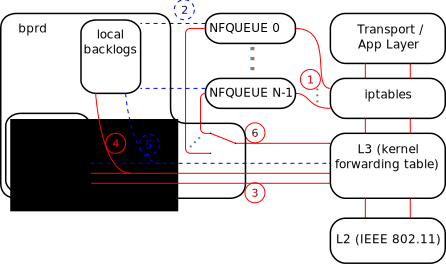
\includegraphics[width=\textwidth]{img/systemdiagram.pdf}
	\caption{A system diagram of \bprd and the networking stack.  Red arrows indicate packet flows and blue arrows
    indicate information flow.}
	\label{fig:systemdiagram}
\end{figure}


\paragraph{\backlogger} The \backlogger\ thread is responsible for filtering and tracking commodity traffic \circled{5}.
Upon startup, the thread issues \iptables\ commands for each commodity.
These commands intercept all packets belonging to the commodity, regardless of whether they have arrived via a network interface or have been generated by local processes.
The filtered packets are directed to an \nfqueue\ queue unique to each commodity \circled{1}.
This filtering and enqueueing is performed in the kernel.
The thread uses the \libnetfilterqueue\ API to interface with the \nfqueue s.
A callback function is registered with \libnetfilterqueue\ to handle the arrival of a commodity packet to an \nfqueue.
Instead of storing whole packets in userspace, a unique ID for each enqueued packet is stored within the thread and the number of packets enqueued for each commodity is updated \circled{2}.


\paragraph{\helloreader} The \helloreader\ thread is responsible for processing control packets, called hello messages, received from neighboring stations \circled{3}.
The \bprd process maintains a commodity list, a bidirectionality flag, and timestamp for each neighboring station.
Every time a hello message is received from a neighbor, \libpacketbb\ is used to extract the fields from the serialized payload.
The commodity list and bidirectionality flag are updated as specifed in the overview and the neighbor's timestamp is updated to the current time.
The timestamp is used by the \hellowriter\ thread to detect when connectivity to a neighbor has dropped.


\paragraph{\hellowriter} The \hellowriter\ thread is responsible for periodically broadcasting the station's commodity levels and neighbor list in the form of control packets called hello messages \circled{4}.
The frequency with which hello messages are sent is controlled by the parameter: \hellointerval.
By default, hello messages are sent once per second.
Prior to constructing a hello message, the \bprd process refreshes its neighbor table and removes any neighbor who has not been updated for five or more \hellointerval s by checking the neighbor entry's timestamp.
Hello messages are then constructed using \libpacketbb, which serializes the data structures used to store backlogs and neighbors into a packet payloads.
Hello messages are transmitted to a well-defined MANET link-local routers multicast address: \(224.0.0.109\) (see RFC 5498 \cite{manet-iana-rfc}).
By sending hello messages via a multicast address, the protocol avoids requiring a unicast copy of a hello message for each neighbor and avoids having to know the list of neighbors ahead of time.


\paragraph{\router} The \router\ thread is responsible for periodically updating the station's routing table based on the station's backlog levels and its neighbors backlog levels \circled{5}.
The frequency with which the routing table is updated is controlled by the parameter: \updateinterval.
By default, routing table updates are performed once per second.
For each defined commodity, the thread finds the neighbor associated with the largest backlog differential and updates the kernel's routing table using \libnlroute.


\paragraph{Main} The main thread periodically selects a commodity with the largest backlog differential (across all neighbors) and releases a packet from the corresponding \nfqueue\ back to the kernel's networking stack \circled{6}, where its next hop is determined by the routing table and is then sent down to the MAC layer for transmission.
The \libnetfilterqueue\ library is used to accomplish this task.
The frequency with which packets are released is controlled by the parameter: \releaseinterval.
By default, packets are released once per second.


%==============================================================================
\subsubsection{Timers}

As introduced above, there are three main timers that affect the operation of \bprd.
The \hellointerval\ controls how frequently the \bprd process sends/receives information to/from its neighbors, \circled{4} and \circled{3} respectively.
The \updateinterval\ controls how frequently backlog information is used to update the routing table \circled{5}.
The \releaseinterval\ controls how frequently packets are released back to the kernel for forwarding \circled{6}.
In general, there are several guidelines for setting these parameters.
For one, packets should be released at a rate equal to or higher than the routes are updated.
It does not make sense to update routes quicker than packets can use them, because a fraction of the routing updates wouldn't be used forward packets.
Second, routes should be updated at a rate equal to or higher than hello messages are received.
It does not make sense to send/receive hello messages at a faster rate than routes are updated - the information contained in the additional hello messages goes to waste.
Summarizing, when configuring \bprd, one might adhere to the following ordering of intervals:
%
\begin{equation}
  \releaseinterval \leq \updateinterval \leq \hellointerval.
\end{equation}


%==============================================================================
\section{Sample Experimental Setup}\label{sec:sample-experiment}

The following paragraphs describe a sample experimental setup for evaluating the performance of \bprd.
Discussed are:
i) the network testbed topology; 
ii) the traffic generation; 
iii) the configuration of \bprd, and; 
iv) the tools used for traffic measurements.


%==============================================================================
\subsection{Network Testbed Topology}

Figure~\ref{fig:linear} shows how the network testbed was setup for our validation experiments.
The SBCs were physically arranged in a line with each node approximately \(30\)~cm apart and connected to a control PC over Ethernet.
This allowed us to control and collect data from each node without affecting the experiments being run on the wireless network.
For each node, a \(20\)~dB attenuator was placed in the RF chain between the wireless card and the antenna.
By configuring the wireless cards to only transmit at \(54\)~Mbps and appropriately setting the transmit power (see Appendix~\ref{sec:topology} and Figure~\ref{fig:linear}), we enforced a linear topology such that a node was able to only communicate with its neighbors (i.e., alix2 was only able to Tx/Rx with alix1 and alix3 and was unable to Tx/Rx with alix0 or alix4).
Traffic from alix0 had to be routed through alix1, alix2, and alix3 in order to reach alix4.
%
\begin{figure}[!ht]
	\centering
	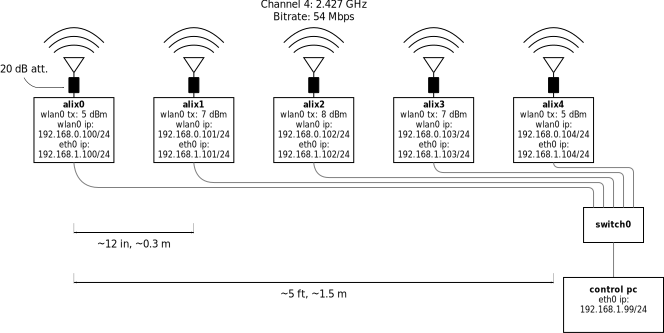
\includegraphics[width=\textwidth]{img/linear.pdf}
	\caption{A sample linear network testbed topology using five ALIX.3D3 stations.}
	\label{fig:linear}
\end{figure}


%==============================================================================
\subsection{\bprd Configuration}

For \bprd, we configured experimental runs with all three timers set to either \(10\)~ms or \(5\)~ms.
That is, for one experimental run, each node running \bprd would: 
i) multicast hello message (which contained the backlog information) every \(\hellointerval=10\)~ms; 
ii) calculate new routes every \(\updateinterval=10\)~ms, and; 
iii) released a queued commodity packet every \(\releaseinterval=10\)~ms.
For the second experimental run, all three timers were set to \(5\)~ms.
These values were selected with the intent that \bprd would introduce only a moderate amount of additional delay for the traffic while not overloading the network with hello messages or over-taxing the CPU of the nodes.



%==============================================================================
\subsection{Traffic Generation/Measurement}

We configured \ditg to generate a UDP flow from alix0 to alix4 with a constant packet size and constant inter-departure time.
The packet size was fixed at \(1024\)~bytes in order to be below the Maximum Transmission Unit (MTU) of \(1500\)~bytes and avoid IP layer fragmentation.
The packet inter-departure time was fixed at \(13.3\)~ms; slightly above the configured \releaseinterval for \bprd.
With this selection of parameters, the configured flow should theoretically have a throughput of \(614.4\)~kbps.


As previously mentioned, \ditg provides the ability to measure the bitrate, delay, and packet loss of generated traffic flows.
In addition to this data, we utilized packet traces taken at each node to measure the throughput as seen by each wireless card, including the relay nodes.
The log file maintained by \bprd was also used to measure the congestion gradient in the network.


%==============================================================================
\section{Future Work}\label{sec:future}

We foresee several directions for future work in extending \bprd:
%
\begin{myitemize}
  \item Extensive exploration of the effect of \bprd timers on network delay and throughput,
  \item Support for forwarding IPv6 packets,
  \item Comparison with extablished mesh/routing protocol, such as BATMAN Advanced, OLSR, and AODV,
  \item Consideration of other topologies (multi-route) and configurations (multi-commodity) of \bprd,
  \item Coordinated operation over multiple network interfaces, and
  \item Last-In-First-Out (LIFO) queueing policy which may yield improved delay \cite{HuaMoeNee2011}.
\end{myitemize}

Finally, the methods discussed in Appendix~\ref{sec:topology} to control the network topology were very useful.
However, these techniques largely required repeated manual tuning.
We see great benefit in developing automated tools to observe and enforce desired wireless topologies.


\bibliographystyle{ieeetr}
\bibliography{refs}

\appendix


%==============================================================================
\section{Topology Control}\label{sec:topology}

Testing \bprd in a shared wireless medium requires some effort to avoid a full-mesh network topology at practical distances.
In this section, we first characterize the wireless environment using a simple model and then describe the effect of several techniques to establish partially connected topologies within the space of a small lab.


%==============================================================================
\subsection{Model}\label{sec:topo-model}

Let \(d(p,q)\) represent the Euclidean distance between points \(p\) and \(q\).
The received power, or received-signal-strength-indication (RSSI), of the signal originating at \(p\) measured at point \(q\) can be modeled as:

\begin{equation}
\rssi(p,q) = P_tG_tG_r\left(\frac{\lambda}{4\pi d(p,q)}\right)^{\alpha} \quad (\textrm{Watts}),
\label{eq:friis}
\end{equation}
%
where \(P_t\) is the transmitted power, \(G_t\) and \(G_r\) are the antenna gains of the transmitter and receiver (located at \(p\) and \(q\)), respectively, \(\lambda\) is the wavelength of the transmitted RF signal, and \(\alpha\) represents the pathloss exponent.


For the time being, we ignore the effects of interference generated by surrounding stations and look to characterize requirements for successful reception of a signal originating at point \(p\).
A common performance metric of wireless hardware is a minimum RSSI \(\beta\), assuming Additive-White-Gaussian-Noise (AWGN), required to achieve a specified QoS often given in terms of a desired frame error rate (FER) or bit error rate (BER).

\begin{equation}
\rssi(p,q) \geq \beta.
\label{eq:rssi-req}
\end{equation}


The minimum required RSSI depends on the hardware in use as well as the modulation and coding scheme in place.
However, for non-spread spectrum schemes, it is at least the thermal noise floor, approximated by the following:
%
\begin{equation}
\beta \geq N = k_BTB \quad (\textrm{Watts}),
\label{eq:noise}
\end{equation}
%
where \(k_B \approx 1.3806\times10^{-23}\)~J/K is the Boltzmann constant, \(T\) is the ambient temperature in Kelvin, and \(B\) is the bandwidth of the channel in Hertz.


Note that the RSSI requirement (\ref{eq:friis}) and (\ref{eq:rssi-req}) can be easily rearranged to compute a maximum distance constraint required for successful communication of a signal originating at point \(p\):
%
\begin{equation}
d(p,q) \leq \frac{\lambda}{4\pi}\sqrt[\alpha]{\frac{P_tG_tG_r}{\beta}} \quad (\textrm{meters}).
\label{eq:dmax}
\end{equation}


In dB scale, (\ref{eq:dmax}) becomes:
%
\begin{equation}
d(p,q) \leq 10^{\frac{P_t + G_t + G_r + \alpha 10 \log_{10}(\frac{\lambda}{4\pi}) - \beta}{\alpha 10}} \quad
(\textrm{meters}),
\label{eq:dmax-dB}
\end{equation}
%
where \(P_t\), \(G_t\), \(G_r\), and \(\beta\) are now in dB units.
(\ref{eq:dmax}) and (\ref{eq:dmax-dB}) serve as an upper bound on the communication range of a station/node located at point \(p\).


Default equipment and operating parameters of IEEE~802.11 networks can yield communication ranges of up to \(300\)~meters and beyond.
Regarding our SBC hardware, we have antennas with a fixed gain \(G_t = G_r = 5\)~dB.
We can tune the transmit power (\(P_t\)), frequency (affecting \(\lambda\)), and bitrate (affecting \(\beta\)) using software --- for now, we assume nominal values of \(P_t = 25\)~dBm max is (\(27\)~dBm), \(\lambda \approx 0.1244\)~meters (\(2.412\)~GHz), and
\(\beta = -95\)~dBm (\(1\)~Mbps).
If we make an assumption about the operating environment surrounding the testbed, \(\alpha = 3\), it follows that \(d(p,q) \leq 215\)~meters.
Thus, without some form of topology control, a testbed of ALIX.3D3 boards deployed within a small laboratory environment will likely be fully connected.
We seek to control this bound in the next section.


%==============================================================================
\subsection{Techniques}\label{sec:topo-techniques}

Avoiding full-mesh network topologies can be accomplished by decreasing the effective range (\ref{eq:dmax}) of each station/node in the network using a combination of techniques:


\begin{myitemize}

\item \textbf{Hardware RF Attenuators}:
  At its simplest, an RF attenuator is a two-port device that accepts an input signal on one port and outputs a reduced-amplitude (\emph{attenuated}) copy of the signal on the other port.
  The gain/loss of the attenuator dictates the degree to which the input signal is attenuated.
  We procured RF attenuators from Mini-Circuits (model VAT-20+) with specifications: \(20\)~dB, \(0.5\)~Watt, \(DC\)-\(6\)~GHz.  These attenuators are rated to handle the output power of the Atheros wireless cards (\(\leq 27\)~dBm) and cover both the \(2.4\)~GHz and \(5\)~GHz bands of the IEEE~802.11 specification.
  By placing one attenuator in each ALIX.3D3 RF chain, we effectively reduce the received signal strength by \(40\)~dB.
  Recalling (\ref{eq:dmax}), the attenuators decrease \(G_t\) and \(G_r\) respectively, and thereby reduce the communication range of each station in the network.
  For our previous example, changing \(G_t = G_r = -15\)~dB yields the bound \(d \leq 10\)~meters.


\item \textbf{Software Power Control}:
  The Linux-based Atheros drivers available within Ubuntu allow the wireless card's transmission power to be adjusted from \(0\)~dBm to \(27\)~dBm in \(1\)~dBm increments.
  Changing the transmission power can be accomplished using the command: \emph{iwconfig wlan0 txpower \#}.
  It follows that decreasing the transmit power \(P_t\) will decrease the range of the station.
  If we change \(P_t = 0\)~dBm, in addition to the RF attenuators, the example communication range decreases further to \(d \leq 1.5\)~meters.


\item \textbf{IEEE~802.11 Bitrate}:
  The Linux-based Atheros drivers also allow the wireless card's bitrate to be adjusted from amongst the available IEEE~802.11a/b/g data rates ranging from \(1\)~Mbps to \(54\)~Mbps.
  Changing the bitrate can be accomplished using the command: \emph{iw wlan0 set bitrates legacy-2.4 \#}.
  As the data rate increases, the minimum RSSI required for successful communication increases.
  For example, at IEEE~802.11b \(1\)~Mbps the RSSI required at room temperature is \(-97\)~dBm, while the IEEE~802.11g \(54\)~Mbps rate requires \(-74\)~dBm at room temperature \cite{dcma82}.
  By forcing higher data rates to be used, the communication range in (\ref{eq:dmax}) can be brought down further.
  In addition to attenuators and power control, enforcing \(54\)~Mbps causes the example communication range to drop to \(d \leq 0.3\)~meters.


\item \textbf{IEEE~802.11 Channel}:
  Finally, the Linux-based Atheros drivers also allow the wireless card to be configured to operate over the IEEE~802.11b/g \(2.4\)~GHz band (11 available \(22\)~MHz-wide channels) or the IEEE~802.11a \(5\)~GHz band (12 available \(22\)~MHz-wide channels).
  By choosing the channel with the largest center frequency (\(5.825\)~GHz), we can decrease \(\lambda\) and the resulting communication range.
  In our example, the communication range would be approximately \(d \leq 0.15\)~meters.

\end{myitemize}


By combining several of the above techniques, we have been able to establish links between stations that are valid up to a fraction of a meter.
This allows us to conduct experiments on a variety of different topologies in a reasonably small geographic area, such as a lab table.

\end{document}
